\typeout{************************************************}
\typeout{Chapter 10 Intermediate and Extreme Values}
\typeout{************************************************}
%
\begin{chapterptx}{Intermediate and Extreme Values}{}{Intermediate and Extreme Values}{}{}{x:chapter:IVTandEVT}
	%
	%
	\typeout{************************************************}
	\typeout{Section 10.1 Completeness of the Real Number System}
	\typeout{************************************************}
	%
	\begin{sectionptx}{Completeness of the Real Number System}{}{Completeness of the Real Number System}{}{}{x:section:IVTandEVT-Completeness}
		Recall that in deriving the Lagrange and Cauchy forms of the remainder for Taylor series, we made use of the Extreme Value Theorem (\terminology{EVT}) and Intermediate Value Theorem (\terminology{IVT}). In \hyperref[x:chapter:Continuity]{Chapter~{\xreffont\ref{x:chapter:Continuity}}}, we produced an analytic definition of continuity that we can use to prove these theorems. To provide the rest of the necessary tools we need to explore the make-up of the real number system. To illustrate what we mean, suppose that we only used the rational number system. We could still use our definition of continuity and could still consider continuous functions such as \(f(x)=x^2\). Notice that \(2\) is a value that lies between \(f(1)=1\)and \(f(2)=4\).%
		\begin{image}{0.315}{0.37}{0.315}%
			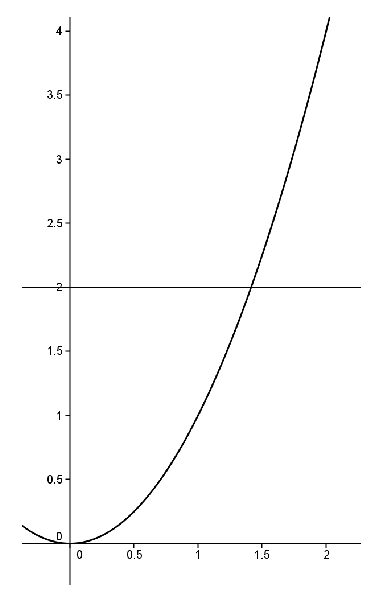
\includegraphics[width=\linewidth]{external/images/Ch6fig1.png}
		\end{image}%
		The IVT says that somewhere between \(1\) and \(2\), \(f\) must take on the value \(2\). That is, there must exist some number \(c\in[1,2]\) such that \(f(c)=2\). You might say, ``Big deal! Everyone knows \(c=\sqrt{2}\) works.''%
		\par
		However, we are only working with rational numbers and \(\sqrt{2}\) \(\)is not rational. As we saw in \hyperref[x:chapter:NumbersRealRational]{Chapter~{\xreffont\ref{x:chapter:NumbersRealRational}}} the rational number system has holes in it, whereas the real number system doesn't. Again, ``Big deal! Let's just say that the real number system contains (square) roots.''%
		\par
		This sounds reasonable and it actually works for square roots, but consider the function \(f(x)=x-\cos x\). We know this is a continuous function. We also know that \(f(0)=-1\) and \(f(\frac{\pi}{2})=\frac{\pi}{2}\). According to the IVT, there should be some number \(c\in[\,0,\frac{\pi}{2}]\), where \(f(c)=0\). The graph is below.%
		\begin{image}{0.315}{0.37}{0.315}%
			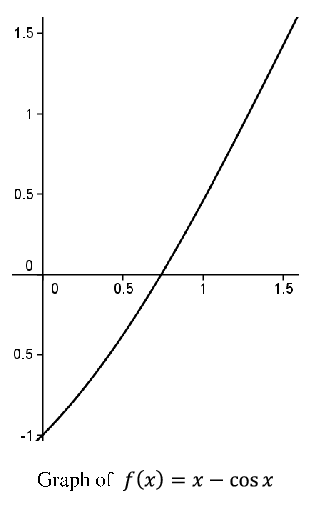
\includegraphics[width=\linewidth]{external/images/Ch6fig2.png}
		\end{image}%
		The situation is not as transparent as before. What would this mysterious \(c\) be where the curve crosses the \(x\) axis? Somehow we need to convey the idea that the real number system is a continuum. That is, it has no ``holes'' in it.%
		\par
		How about this? Why don't we just say that it has no holes in it? Sometimes the simple answer works best! But not in this case. How are we going to formulate a rigorous proof based on this statement? Just like with convergence and continuity, what we need is a rigorous way to convey this idea that the real number system does not have any holes, that it is \emph{complete.}%
		\par
		We will see that there are several different, but equivalent ways to convey this notion of completeness. We will explore some of them in this chapter. For now we adopt the following as our \emph{Completeness Axiom} for the real number system.%
		\begin{axiom}{Nested Interval Property of the Real Number System (\terminology{NIP}).}{}{g:axiom:idp238}%
			Suppose we have two sequences of real numbers \(\left(x_n\right)\)and \(\left(y_n\right)\) satisfying the following conditions:%
			\par
			%
			\begin{enumerate}
				\item{}\(x_1\leq x_2\leq x_3\leq\ldots\) (this says that the sequence, \(\left(x_n\right)\), is non-decreasing)%
				\item{}\(y_1\geq y_2\geq y_3\geq\ldots\) (this says that the sequence, \(\left(y_n\right)\), is non-increasing) %
				\item{}\(\forall\) \(n\), \(x_n\leq y_n\)%
				\item{}\(\displaystyle \lim_{n\rightarrow\infty}\left(y_n-x_n\right)=0\)%
			\end{enumerate}
			%
			\par
			Then there exists a unique number \(c\) such that \(x_n\leq
			c\leq y_n\) for all \(n\).%
		\end{axiom}
		Geometrically, we have the following situation.%
		\begin{image}{0.125}{0.75}{0.125}%
			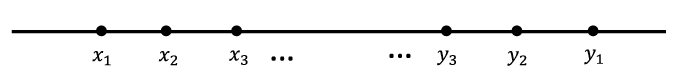
\includegraphics[width=\linewidth]{external/images/Ch6fig3.png}
		\end{image}%
		Notice that we have two sequences \(\left(x_n\right)\) and \(\left(y_n\right)\), one increasing (really non-decreasing) and one decreasing (non-increasing). These sequences do not pass each other. In fact, the following is true:%
		\begin{problem}{}{g:problem:idp239}%
			Let \((x_n), (y_n)\) be sequences as in the NIP. Show that for all \(n, m \in\NN\), \(x_n\le y_m\).%
		\end{problem}
		They are also coming together in the sense that \(\lim_{n\rightarrow\infty}\left(y_n-x_n\right)=0\).  The NIP says that in this case there is a unique real number \(c\) in the middle of all of this \textbackslash{}lbrack \(x_n\leq c\leq y_n\) for all \(n\)\textbackslash{}rbrack.%
		\begin{image}{0.125}{0.75}{0.125}%
			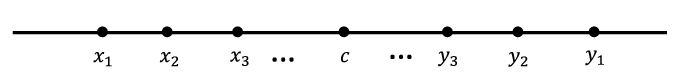
\includegraphics[width=\linewidth]{external/images/Ch6fig4.png}
		\end{image}%
		If there was no such \(c\) then there would be a hole where these two sequences come together.  The NIP guarantees that there is no such hole.  We do not need to prove this since an axiom is, by definition, a self evident truth.  We are taking it on faith that the real number system obeys this law.  The next problem shows that the completeness property distinguishes the real number system from the rational number system.%
		\begin{problem}{}{g:problem:idp240}%
			\begin{enumerate}[font=\bfseries,label=(\alph*),ref=\alph*]
				\item{}Find two sequences of rational numbers \(\left(x_n\right)\)and \(\left(y_n\right)\) which satisfy properties 1-4 of the NIP and such that there is no rational number \(c\) satisfying the conclusion of the NIP.%
				\par\smallskip%
				\noindent\textbf{\blocktitlefont Hint}.\hypertarget{g:hint:idp241}{}\quad{}Consider the decimal expansion of an irrational number.%
				\item{}Find two sequences of rational numbers \(\left(x_n\right)\) and \(\left(y_n\right)\) which satisfy properties 1-4 of the NIP and such that there is a rational number \(c\) satisfying the conclusion of the NIP.%
			\end{enumerate}
		\end{problem}
		You might find the name ``Nested Interval Property'' to be somewhat curious. One way to think about this property is to consider that we have a sequence of ``nested closed intervals'' \([\,x_1,y_1]\supseteq[\,x_2,y_2]\supseteq[\,x_3,y_3]\supseteq\cdots\) whose lengths \(\,y_n-x_n\) are ``shrinking to \(0\).'' The conclusion is that the intersection of these intervals is non-empty and, in fact, consists of a single point. That is, \(\bigcap_{n=1}^\infty[x_n,y_n]=\{c\}\).%
		\par
		It appears that the sequences \(\left(x_n\right)\) and \(\left(y_n\right)\) in the NIP converge to \(c\). This is, in fact, true and can be proven rigorously. In what follows, this will prove to be a valuable piece of information.%
		\begin{theorem}{}{}{x:theorem:thm_ConvergeToC}%
			\index{Nested Interval Property (NIP)!endpoints}\index{limit!of interval endpoints in the NIP} Suppose that we have two sequences \(\left(x_n\right)\) and \(\left(y_n\right)\) satisfying all of the assumptions of the Nested Interval Property. If \(c\) is the unique number such that \(x_n\leq c\leq y_n\) for all \(n\), then \(\lim_{n\rightarrow\infty}x_n=c\) and \(\lim_{n\rightarrow\infty}y_n=c\).%
		\end{theorem}
		\begin{problem}{}{g:problem:idp242}%
			\index{Nested Interval Property (NIP)!endpoints} Prove \hyperref[x:theorem:thm_ConvergeToC]{Theorem~{\xreffont\ref{x:theorem:thm_ConvergeToC}}}.%
		\end{problem}
		To illustrate the idea that the NIP ``plugs the holes'' in the real line, we will prove the existence of square roots of nonnegative real numbers.%
		\begin{theorem}{}{}{x:theorem:thm_SqrtsExist}%
			\index{square roots exist}%
			Suppose \(a\in\mathbb{R},\,a\geq 0\). There exists a real number \(c\geq 0\) such that \(c^2=a\).%
		\end{theorem}
		Notice that we can't just say, ``Let \(c=\sqrt{a}\),'' since the idea is to show that this square root exists. In fact, throughout this proof, we cannot really use a square root symbol as we haven't yet proved that they (square roots) exist. We will give the idea behind the proof as it illustrates how the NIP is used.%
		\begin{proof}{Sketch of Proof.}{g:proof:idp243}
			Our strategy is to construct two sequences which will ``narrow in'' on the number \(c\) that we seek. With that in mind, we need to find a number \(x_1\) such that \(x_1^2\leq a\) and a number \(y_1\) such that \(y_1^2\geq a\). (Remember that we can't say \(\sqrt{x_1}\) or\(\sqrt{y_1}\).) There are many possibilities, but how about \(x_1=0\) and \(y_1=a+1?\) You can check that these will satisfy \(x_1^2\leq a\leq\) \(y_1^2\). Furthermore \(x_1\leq y_1\). This is the starting point.%
			\par
			The technique we will employ is often called a bisection technique, and is a useful way to set ourselves up for applying the NIP. Let \(m_1\) be the midpoint of the interval \([\,x_1,y_1]\). Then either we have \(m_1^2\leq a\) or \(m_1^2\geq a\). In the case \(m_1^2\leq a\), we really want \(m_1\) to take the place of \(x_1\) since it is larger than \(\,x_1\), but still represents an underestimate for what would be the square root of \(a\). This thinking prompts the following move. If \(m_1^2\leq a\), we will relabel things by letting \(x_2=m_1\) and \(y_2=y_1\). The situation looks like this on the number line.%
			\begin{image}{0.22}{0.56}{0.22}%
				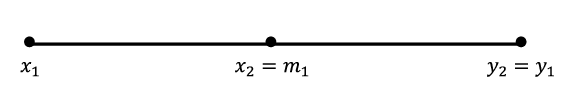
\includegraphics[width=\linewidth]{external/images/Ch6fig5.png}
			\end{image}%
			In the other case where \(a\leq m_1^2\), we will relabel things by letting \(x_2=x_1\) and \(y_2=m_1\). The situation looks like this on the number line.%
			\begin{image}{0.22}{0.56}{0.22}%
				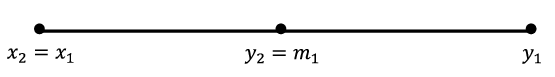
\includegraphics[width=\linewidth]{external/images/Ch6fig6.png}
			\end{image}%
			In either case, we've reduced the length of the interval where the square root lies to half the size it was before. Stated in more specific terms, in either case we have the same results:%
			\begin{equation*}
				x_1\leq x_2\leq y_2\leq y_1;\ \  x_1^2\leq a\leq y_1^2;\ \  x_2^2\leq a\leq y_2^2
			\end{equation*}
			and%
			\begin{equation*}
				y_2-x_2=\frac{1}{2}\left(y_1-x_1\right)\text{.}
			\end{equation*}
			%
			\par
			Now we play the same game, but instead we start with the interval \([x_2,y_2]\). Let \(m_2\) be the midpoint of \([x_2,y_2]\). Then we have \(m_2^2\leq a\) or \(m_2^2\geq a\). If \(m_2^2\leq a\), we relabel \(x_3=m_2\) and \(y_3=y_2\). If \(a\leq m_2^2\), we relabel \(x_3=x_2\) and \(y_3=m_2\). In either case, we end up with%
			\begin{equation*}
				x_1\leq x_2\leq x_3\leq y_3\leq y_2\leq y_1;\ \   x_1^2\leq a\leq y_1^2;\ \  x_2^2\leq a\leq y_2^2;\ \   x_3^2\leq a\leq y_3^2
			\end{equation*}
			and%
			\begin{equation*}
				y_3-x_3=\frac{1}{2}\left(y_2-x_2\right)=\frac{1}{2^2}\left(y_1-x_1\right)\text{.}
			\end{equation*}
			%
			\par
			Continuing in this manner, we will produce two sequences, \(\left(x_n\right)\)and \(\left(y_n\right)\) satisfying the following conditions:%
			\begin{enumerate}
				\item{}\(\displaystyle x_1\leq x_2\leq x_3\leq\ldots\)%
				\item{}\(\displaystyle y_1\geq y_2\geq y_3\geq\ldots\)%
				\item{}\(\forall\) \(n\), \(x_n\leq y_n\)%
				\item{}\(\displaystyle \lim_{n\rightarrow\infty}\left(y_n-x_n\right)=\,\lim_{n\rightarrow\infty}\frac{1}{2^{n-1}}\left(y_1-x_1\right)=0\)%
				\item{}These sequences also satisfy the following property:%
				\begin{equation*}
					\forall n,\,x_n^2\leq a\leq y_n^2
				\end{equation*}
				%
			\end{enumerate}
			%
			\par
			Properties 1-4 tell us that \(\left(x_n\right)\)and \(\left(y_n\right)\) satisfy all of the conditions of the NIP, so we can conclude that there must exist a real number \(c\) such that \(x_n\leq c\leq y_n\) for all \(n\). At this point, you should be able to use property 5. to show that \(c^2=a\) as desired.%
		\end{proof}
		\begin{problem}{}{g:problem:idp244}%
			\index{Nested Interval Property (NIP)!square roots of integers, and}\index{Nested Interval Property (NIP)!implies the existence of square roots of integers} Turn the above outline into a formal proof of \hyperref[x:theorem:thm_SqrtsExist]{Theorem~{\xreffont\ref{x:theorem:thm_SqrtsExist}}}.%
		\end{problem}
		The bisection method we employed in the proof of \hyperref[x:theorem:thm_SqrtsExist]{Theorem~{\xreffont\ref{x:theorem:thm_SqrtsExist}}} is pretty typical of how we will use the NIP, as taking midpoints ensures that we will create a sequence of ``nested intervals.'' We will employ this strategy in the proofs of the IVT and EVT. Deciding how to relabel the endpoints of our intervals will be determined by what we want to do with these two sequences of real numbers. This will typically lead to a fifth property, which will be crucial in proving that the \(c\) guaranteed by the NIP does what we want it to do. Specifically, in the above example, we always wanted our candidate for \(\sqrt{a}\) to be in the interval \([\,x_n,y_n]\). This judicious choice led to the extra Property~5: \(\forall\) \(n,\,x_n^2\leq a\leq y_n^2\). In applying the NIP to prove the IVT and EVT, we will find that properties 1-4 will stay the same. Property~5 is what will change based on the property we want \(c\) to have.%
		\par
		Before we tackle the IVT and EVT, let's use the NIP to address an interesting question about the Harmonic Series. \index{series!Harmonic Series!slow divergence of} Recall that the Harmonic Series, \(1+\frac{1}{2}+\frac{1}{3}+\frac{1}{4}+\cdots\), grows without bound, that is, \(\sum_{n=1}^\infty\frac{1}{n}=\infty\).  The question is how slowly does this series grow?  For example, how many terms would it take before the series surpasses 100? 1000? 10000?  Leonhard Euler \index{Euler, Leonhard} decided to tackle this problem in the following way.  Euler decided to consider the \(\lim_{n\rightarrow\infty}\left(\left(1+\frac{1}{2}+\frac{1}{3}+\cdots+
		\frac{1}{n}\right)-\text{ ln } \left(n+1\right)\right)\).  This limit is called Euler's constant and is denoted by \(\gamma\). This says that for \(n\) large, we have \(1+\frac{1}{2}+\frac{1}{3}+\cdots+\frac{1}{n}\approx\)ln\(\left(n+1\right)+\gamma\). If we could approximate \(\gamma\), then we could replace the inequality \(1+\frac{1}{2}+\frac{1}{3}+\cdots+\frac{1}{n}\geq
		100\) with the more tractable inequality ln\(\left(n+1\right)+\gamma\) \(\geq 0\) and solve for \(n\) in this.  This should tell us roughly how many terms would need to be added in the Harmonic Series to surpass 100. Approximating \(\gamma\) with a computer is not too bad.  We could make \(n\) as large as we wish in \(\left(1+\frac{1}{2}+\frac{1}{3}+\cdots+\frac{1}{n}\right)-\)ln\(\left(1+n\right)\) to make closer approximations for \(\gamma\).  The real issue is, \alert{HOW DO WE KNOW THAT}%
		\begin{equation*}
			\lim_{n\rightarrow\infty}\left(\left(1+\frac{1}{2}+\frac{1}{3}+\cdots+\frac{1}{n}\right)-\text{ ln } \left(\text{n} +1\right)\right)
		\end{equation*}
		\alert{ACTUALLY EXISTS?}%
		\par
		You might want to say that obviously it should, but let us point out that as of the printing of this book (2013), it is not even known if \(\gamma\) is rational or irrational. So, in our opinion the existence of this limit is not so obvious. This is where the NIP will come into play; we will use it to show that this limit, in fact, exists. The details are in the following problem.%
		\begin{problem}{}{g:problem:idp245}%
			The purpose of this problem is to show that%
			\begin{equation*}
				\lim_{n\rightarrow\infty}\left(\left(1+\frac{1}{2}+\frac{1}{3}+\cdots+ \frac{1}{n}\right)-\ln\left(n+1\right)\right)
			\end{equation*}
			exists.%
			\begin{enumerate}[font=\bfseries,label=(\alph*),ref=\alph*]
				\item{}Let \(x_n=\left(1+\frac{1}{2}+\frac{1}{3}+\cdots+\frac{1}{n}\right)-\ln\left(n+1 \right)\). Use the following diagram to show%
				\begin{equation*}
					x_1\leq x_2\leq x_3\leq\cdots
				\end{equation*}
				%
				\begin{image}{0.08}{0.84}{0.08}%
					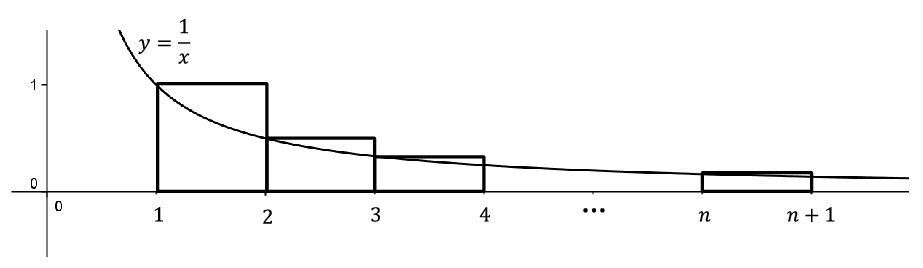
\includegraphics[width=\linewidth]{external/images/Ch6fig7.png}
				\end{image}%
				\item{}Let \(z_n=\ln\left(n+1\right)-\left(\frac{1}{2}+\frac{1}{3}+\cdots+\frac{1}{n+1} \right)\). Use a similar diagram to show that \(z_1\leq z_2\leq z_3\leq\cdots\).%
				\item{}Let \(y_n=1-z_n\).  Show that \(\left(x_n\right)\) and \(\left(y_n\right)\) satisfy the hypotheses of the nested interval property and use the NIP to conclude that there is a real number \(\gamma\) such that \(x_n\leq\gamma\leq
				y_n\) for all \(n\).%
				\item{}Conclude that \(\lim_{n\rightarrow\infty}\left(\left(1+\frac{1}{2}+\frac{1}{3}+\cdots+
				\frac{1}{n}\right)-\ln\left(n+1\right)\right)=\gamma\).%
			\end{enumerate}
		\end{problem}
		\begin{problem}{}{g:problem:idp246}%
			Use the fact that \(x_n\leq\gamma\leq y_n\) for all \(n\) to approximate \(\gamma\) to three decimal places.%
		\end{problem}
		\begin{problem}{}{g:problem:idp247}%
			\begin{enumerate}[font=\bfseries,label=(\alph*),ref=\alph*]
				\item{}Use the fact that for large \(n\), \(1+\frac{1}{2}+\frac{1}{3}+\cdots+\frac{1}{n}\approx
				\ln\left(n+1\right)+ \gamma\) to determine approximately how large \(n\) must be to make%
				\begin{equation*}
					1+\frac{1}{2}+\frac{1}{3}+\cdots+\frac{1}{n}\geq 100\text{.}
				\end{equation*}
				%
				\item{}Suppose we have a supercomputer which can add 10 trillion terms of the Harmonic Series per second. Approximately how many earth lifetimes would it take for this computer to sum the Harmonic Series until it surpasses 100?%
			\end{enumerate}
		\end{problem}
	\end{sectionptx}
	%
	%
	\typeout{************************************************}
	\typeout{Section 10.2 Proof of the Intermediate Value Theorem}
	\typeout{************************************************}
	%
	\begin{sectionptx}{Proof of the Intermediate Value Theorem}{}{Proof of the Intermediate Value Theorem}{}{}{x:section:IVTandEVT-ProofOfIVT}
		We now have all of the tools to prove the Intermediate Value Theorem (\terminology{IVT}).%
		\begin{theorem}{}{}{x:theorem:IntermediateValueTheorem}%
			\terminology{Intermediate Value Theorem}%
			\par
			\index{Intermediate Value Theorem (IVT)} Suppose \(f(x)\) is continuous on \([a,b]\) and \(v\) is any real number between \(f(a)\) and \(f(b)\). Then there exists a real number \(c\in[\,a,b]\) such that \(f(c)=v\).%
		\end{theorem}
		\begin{proof}{Sketch of Proof.}{g:proof:idp248}
			We have two cases to consider: \(f(a)\leq v\leq f(b)\) and \(f(a)\geq v\geq f(b)\).%
			\par
			We will look at the case \(f(a)\leq v\leq f(b)\). Let \(x_1=a\) and \(y_1=b\), so we have \(x_1\leq y_1\) and \(f(x_1)\leq v\leq f(y_1)\). Let \(\,m_1\) be the midpoint of \([\,x_1,y_1]\) and notice that we have either \(f(m_1)\leq v\) or \(f(m_1)\geq v\). If \(f(m_1)\leq v\) , then we relabel \(x_2=m_1\) and \(y_2=y_1\). If \(f(m_1)\geq v\) , then we relabel \(x_2=x_1\) and \(y_2=m_1\). In either case, we end up with \(x_1\leq x_2\leq y_2\leq y_1\), \(y_2-x_2=\frac{1}{2}\left(y_1-x_1\right)\), \(f(x_1)\leq v\leq f(y_1)\), and \(f(x_2)\leq v\leq f(y_2)\).%
			\par
			Now play the same game with the interval \([\,x_2,y_2]\). If we keep playing this game, we will generate two sequences \(\left(x_n\right)\) and \(\left(y_n\right)\), satisfying all of the conditions of the nested interval property. These sequences will also satisfy the following extra property: \(\forall\) \(n,\,f(x_n)\leq v\leq f(y_n)\). By the NIP, there exists a \(c\) such that \(\,x_n\leq c\leq y_n\), \(\forall\) \(n\). This should be the \(c\) that we seek though this is not obvious. Specifically, we need to show that \(f(c)=v\). This should be where the continuity of \(f\) at \(c\) and the extra property on \(\left(x_n\right)\)and \(\left(y_n\right)\) come into play.%
		\end{proof}
		\begin{problem}{}{g:problem:idp249}%
			\index{Intermediate Value Theorem (IVT)!the case \(f(a)\leq v\leq f(b)\)} Turn the ideas of the previous paragraphs into a formal proof of the IVT for the case \(f(a)\leq v\leq f(b)\).%
		\end{problem}
		\begin{problem}{}{g:problem:idp250}%
			\index{Intermediate Value Theorem (IVT)!the case \(f(a)\geq v\geq f(b)\)} We can modify the proof of the case \(f(a)\leq v\leq f(b)\) into a proof of the IVT for the case \(f(a)\geq v\geq f(b)\). However, there is a sneakier way to prove this case by applying the IVT to the function \(-f\). Do this to prove the IVT for the case \(f(a)\geq v\geq f(b)\).%
		\end{problem}
		\begin{problem}{}{g:problem:idp251}%
			\index{polynomials!with odd degree must have a root}\index{Intermediate Value Theorem (IVT)!a polynomial with odd degree must have a root} Use the IVT to prove that any polynomial of odd degree must have a real root.%
		\end{problem}
	\end{sectionptx}
	%
	%
	\typeout{************************************************}
	\typeout{Section 10.3 The Bolzano-Weierstrass Theorem}
	\typeout{************************************************}
	%
	\begin{sectionptx}{The Bolzano-Weierstrass Theorem}{}{The Bolzano-Weierstrass Theorem}{}{}{x:section:IVTandEVT-BWT}
		Once we introduced the Nested Interval Property, the Intermediate Value Theorem followed pretty readily. The proof of Extreme Value (which says that any continuous function \(f\)defined on a closed interval \([\,a,b]\) must have a maximum and a minimum) takes a bit more work. First we need to show that such a function is bounded.%
		\begin{theorem}{}{}{x:theorem:thm_CompactBounded}%
			\index{continuous functions!continuous function on a closed, bounded interval is bounded} A continuous function defined on a closed, bounded interval must be bounded.  That is, let \(f\) be a continuous function defined on \([\,a,b]\).  Then there exists a positive real number \(B\) such that \(|f(x)|\leq B\) for all \(x\in[\,a,b]\).%
		\end{theorem}
		\alert{Sketch of Alleged Proof:} Let's assume, for contradiction, that there is no such bound \(B\). This says that for any positive integer \(n\), there must exist \(x_n\in[a,b]\) such that \(\abs{f(x_n)}>n\). (Otherwise \(n\) would be a bound for \(f\).) \alert{IF} the sequence \(\left(x_n\right)\) converged to something in \([\,a,b]\), say \(c\), then we would have our contradiction. Indeed, we would have \(\lim_{n\rightarrow\infty}x_n=c\). By the continuity of \(f\) at \(c\) and \hyperref[x:theorem:thm_LimDefOfContinuity]{Theorem~{\xreffont\ref{x:theorem:thm_LimDefOfContinuity}}} of \hyperref[x:chapter:Continuity]{Chapter~{\xreffont\ref{x:chapter:Continuity}}}, we would have \(\lim_{n\rightarrow\infty}f(x_n)=f(c)\). This would say that the sequence \(\left(f(x_n)\right)\) converges, so by \hyperref[x:lemma:lemma_BoundedConvergent]{Lemma~{\xreffont\ref{x:lemma:lemma_BoundedConvergent}}} of \hyperref[x:chapter:Convergence]{Chapter~{\xreffont\ref{x:chapter:Convergence}}}, it must be bounded. This would provide our contradiction, as we had \(|f(x_n)|>n\), for all positive integers \(n\). \alert{QED?}%
		\par
		This would all work well except for one little problem. The way it was constructed, there is no reason to expect the sequence \(\left(x_n\right)\) to converge to anything and we can't make such an assumption. That is why we emphasized the \alert{IF} above. Fortunately, this idea can be salvaged. While it is true that the sequence \(\left(x_n\right)\) may not converge, part of it will. We will need the following definition.%
		\begin{definition}{}{x:definition:def_subsequences}%
			\index{sequences!subsequences} Let \(\left(n_k\right)_{k=1}^\infty\) be a strictly increasing sequence of positive integers; that is, \(n_1\lt n_2\lt n_3\lt \cdots\) . If \(\left(x_n\right)_{n=1}^\infty\)is a sequence, then \(\left(x_{n_k}\right)_{k=1}^\infty=\left(x_{n_1},x_{n_2},x_{n_3},\ldots \right)\) is called a \textbraceleft{}subsequence\textbraceright{} of \(\left(x_n\right)\).%
		\end{definition}
		The idea is that a subsequence of a sequence is a part of the sequence, \((x_n)\), which is itself a sequence. However, it is a little more restrictive. We can choose any term in our sequence to be part of the subsequence, but once we choose that term, we can't go backwards. This is where the condition \(n_1\lt n_2\lt n_3\lt \cdots\) comes in. For example, suppose we started our subsequence with the term \(x_{100}\). We could not choose our next term to be \(x_{99}\). The subscript of the next term would have to be greater than 100. In fact, the thing about a subsequence is that it is all in the subscripts; we are really choosing a subsequence \(\left(n_k\right)\) of the sequence of subscripts \(\left(n\right)\) in \(\left(x_n\right)\).%
		\begin{example}{}{g:example:idp252}%
			Given the sequence \(\left(x_n\right)\), the following are subsequences.%
			\begin{enumerate}[font=\bfseries,label=(\alph*),ref=\alph*]
				\item{}\(\left(x_2,\,x_4,\,x_6,\,\ldots\right)=\left(x_{2k}\right)_{k=1}^\infty\)%
				\item{}\(\left(x_1,\,x_4,\,x_9,\,\ldots\right)=\left(x_{k^2}\right)_{k=1}^ \infty\)%
				\item{}\(\left(x_n\right)\) itself.%
			\end{enumerate}
		\end{example}
		\begin{example}{}{g:example:idp253}%
			The following are NOT subsequences.%
			\begin{enumerate}[font=\bfseries,label=(\alph*),ref=\alph*]
				\item{}\(\left(x_1,\,x_1,\,x_1,\,\ldots\right)\)%
				\item{}\(\left(x_{99},\,x_{100},\,x_{99},\,\ldots\right)\)%
				\item{}\(\left(x_1,\,x_2,\,x_3\right)\)%
			\end{enumerate}
		\end{example}
		The subscripts in the examples we have seen so far have a discernable pattern, but this need not be the case. For example,%
		\begin{equation*}
			\left(x_2,\,x_5,\,x_{12},\,x_{14},\,x_{23},\,\ldots\right)
		\end{equation*}
		would be a subsequence as long as the subscripts form an increasing sequence themselves.%
		\begin{problem}{}{g:problem:idp254}%
			\index{sequences!all subsequences of a convergent sequence converge} Suppose \(\lim_{n\rightarrow\infty}x_n=c\). Prove that \(\lim_{k\rightarrow\infty}x_{n_k}=c\) for any subsequence \(\left(x_{n_k}\right)\) of \(\left(x_n\right)\).%
			\par\smallskip%
			\noindent\textbf{\blocktitlefont Hint}.\hypertarget{g:hint:idp255}{}\quad{}\(n_k\geq k\).%
		\end{problem}
		A very important theorem about subsequences was introduced by Bernhard Bolzano \index{Bolzano, Bernhard} and, later, independently proven \index{Weierstrass, Karl} by Karl Weierstrass. Basically, this theorem says that any bounded sequence of real numbers has a convergent subsequence.%
		\begin{theorem}{}{}{x:theorem:BolzanoWeierstrass}%
			\alert{The Bolzano-Weierstrass Theorem}%
			\par
			\index{Bolzano-Weierstrass Theorem} Let \(\left(x_n\right)\) be a sequence of real numbers such that \(x_n\in[\,a,b]\), \(\forall\) \(n\).  Then there exists \(c\in[\,a,b]\) and a subsequence \(\left(x_{n_k}\right)\), such that \(\lim_{k\rightarrow\infty}x_{n_k}=c\).%
		\end{theorem}
		As an example of this theorem, consider the sequence%
		\begin{equation*}
			\left((-1)^n\right)=\left(-1,1,-1,1,\ldots\right) \text{.}
		\end{equation*}
		%
		\par
		This sequence does not converge, but the subsequence%
		\begin{equation*}
			\left((-1)^{2k}\right)=\left(1,1,1,\ldots\right)
		\end{equation*}
		converges to \(1\). This is not the only convergent subsequence, as \(\left((-1)^{2k+1}\right)=(-1,-1,-1,\,\ldots)\) converges to \(-1\). Notice that if the sequence is unbounded, then all bets are off; the sequence may have a convergent subsequence or it may not. The sequences \(\left(\left((-1)^n+1\right)n\right)\) and \(\left(n\right)\) represent these possibilities as the first has, for example, \(\left(\left((-1)^{2k+1}+1\right)(2k+1)\right)=(0,0,0,\,\ldots)\) and the second one has none.%
		\par
		The Bolzano-Weierstrass Theorem says that no matter how ``random'' the sequence \(\left(x_n\right)\) may be, as long as it is bounded then some part of it must converge. This is very useful when one has some process which produces a ``random'' sequence such as what we had in the idea of the alleged proof in \hyperref[x:theorem:thm_CompactBounded]{Theorem~{\xreffont\ref{x:theorem:thm_CompactBounded}}}.%
		\begin{proof}{Sketch of a Proof of the Bolzano-Weierstrass Theorem.}{g:proof:idp256}
			Suppose we have our sequence \(\left(x_n\right)\) such that \(x_n\in[a,b]\), \(\forall\) \(n\). To find our \(c\) for the subsequence to converge to we will use the NIP. Since we are already using \(\left(x_n\right)\) as our original sequence, we will need to use different letters in setting ourselves up for the NIP. With this in mind, let \(a_1=a\) and \(b_1=b\), and notice that \(x_n\in[a_1,b_1]\) for infinitely many \(n\). (This is, in fact true for all \(n\), but you'll see why we said it the way we did.) Let \(m_1\) be the midpoint of \([a_1,b_1]\) and notice that either \(x_n\in[a_1,m_1]\) for infinitely many \(n\) or \(x_n\in[m_1,b_1]\) for infinitely many \(n\). If \(x_n\in[a_1,m_1]\) for infinitely many \(n\), then we relabel \(a_2=a_1\) and \(b_2=m_1\). If \(x_n\in[m_1,b_1]\) for infinitely many \(n\), then relabel \(a_2=m_1\) and \(b_2=b_1\). In either case, we get \(a_1\leq a_2\leq b_2\leq b_1\), \(b_2-a_2=\frac{1}{2}\left(b_1-a_1\right)\), and \(x_n\in[a_2,b_2]\) for infinitely many \(n\).%
			\par
			Now we consider the interval \([a_2,b_2]\) and let \(m_2\) be the midpoint of \([a_2,b_2]\). Since \(x_n\in[a_2,b_2]\) for infinitely many \(n\), then either \(x_n\in[a_2,m_2]\) for infinitely many \(n\) or \(x_n\in[m_2,b_2]\) for infinitely many \(n\). If \(x_n\in[a_2,m_2]\) for infinitely many \(n\), then we relabel \(a_3=a_2\) and \(b_3=m_2\). If \(x_n\in[m_2,b_2]\) for infinitely many \(n\), then we relabel \(a_3=m_2\) and \(b_3=b_2\). In either case, we get \(a_1\leq a_2\leq a_3\leq b_3\leq b_2\leq b_1\), \(b_3-a_3=\frac{1}{2}\left(b_2-a_2\right)=\frac{1}{2^2}\left(b_1-a_1\right)\), and \(x_n\in[a_3,b_3]\) for infinitely many \(n\).%
			\par
			If we continue in this manner, we will produce two sequences \(\left(a_k\right)\)and \(\left(b_k\right)\) with the following properties:%
			\begin{enumerate}
				\item{}\(\displaystyle a_1\leq a_2\leq a_3\leq\cdots\)%
				\item{}\(\displaystyle b_1\geq b_2\geq b_3\geq\cdots\)%
				\item{}\(\forall\) \(k,\,a_k\leq b_k\)%
				\item{}\(\displaystyle \displaystyle\lim_{k\rightarrow\infty}\left(b_k-a_k\right)=\,\lim_{k\rightarrow\infty} \frac{1}{2^{k-1}}\left(b_1-a_1\right)=0\)%
				\item{}For each \(k\), \(x_n\in[\,a_k,b_k]\) for infinitely many \(n\)%
			\end{enumerate}
			%
			\par
			By properties 1-5 and the NIP, there exists a unique \(c\) such that \(c\in[a_k,b_k]\), for all \(k\). In particular, \(c\in[a_1,b_1]=[a,b]\).%
			\par
			We have our \(c\). Now we need to construct a subsequence converging to it. Since \(x_n\in[a_1,b_1]\) for infinitely many \(n\), choose an integer \(n_1\) such that \(x_{n_1}\in[a_1,b_1]\). Since \(x_n\in[a_2,b_2]\) for infinitely many \(n\), choose an integer \(n_2>n_1\) such that \(x_{n_2}\in[a_2,b_2]\). (Notice that to make a subsequence it is crucial that \(n_2>n_1\), and this is why we needed to insist that \(x_n\in[a_2,b_2]\) for infinitely many \(n\).) Continuing in this manner, we should be able to build a subsequence \(\left(x_{n_k}\right)\) that will converge to \(c\). You can supply the details in the following problem.%
		\end{proof}
		\begin{problem}{}{g:problem:idp257}%
			\index{Bolzano-Weierstrass Theorem (BWT)} Turn the ideas of the above outline into a formal proof of the Bolzano-Weierstrass Theorem.%
		\end{problem}
		\begin{problem}{}{g:problem:idp258}%
			\index{Bolzano-Weierstrass Theorem (BWT)!implies that a  continuous functions on a closed set is bounded}\index{continuous functions!on a closed set, and the Bolzano-Weierstrass Theorem}\index{continuity!Bolzano-Weierstrass Theorem implies a continuous function on a closed set is bounded} Use the Bolzano-Weierstrass Theorem to complete the proof of \hyperref[x:theorem:thm_CompactBounded]{Theorem~{\xreffont\ref{x:theorem:thm_CompactBounded}}}.%
		\end{problem}
	\end{sectionptx}
	%
	%
	\typeout{************************************************}
	\typeout{Section 10.4 The Supremum and the Extreme Value Theorem}
	\typeout{************************************************}
	%
	\begin{sectionptx}{The Supremum and the Extreme Value Theorem}{}{The Supremum and the Extreme Value Theorem}{}{}{x:section:IVTandEVT-SupremumAndEVT}
		\hyperref[x:theorem:thm_CompactBounded]{Theorem~{\xreffont\ref{x:theorem:thm_CompactBounded}}} says that a continuous function on a closed, bounded interval must be bounded. Boundedness, in and of itself, does not ensure the existence of a maximum or minimum. We must also have a closed, bounded interval. To illustrate this, consider the continuous function \(f(x)=\)tan\(^{-1}x\) defined on the (unbounded) interval \(\left(-\infty,\infty\right)\).%
		\begin{image}{0.125}{0.75}{0.125}%
			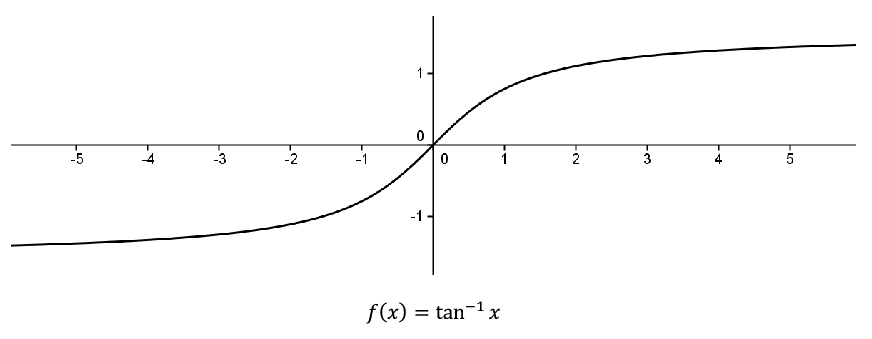
\includegraphics[width=\linewidth]{external/images/Ch6fig8.png}
		\end{image}%
		This function is bounded between \(-\frac{\pi}{2}\)and \(\frac{\pi}{2}\), but it does not attain a maximum or minimum as the lines \(y=\pm\frac{\pi}{2}\) are horizontal asymptotes. Notice that if we restricted the domain to a closed, bounded interval then it would attain its extreme values on that interval (as guaranteed by the \terminology{EVT}).%
		\par
		To find a maximum we need to find the smallest possible upper bound for the range of the function. This prompts the following definitions.%
		\begin{definition}{}{x:definition:def_UpperBound}%
			\index{Upper Bound} Let \(S\subseteq\mathbb{R}\) and let \(b\) be a real number. We say that \(b\) is an upper bound of \(S\) provided \(b\geq x\) for all \(x\in S\).%
		\end{definition}
		For example, if \(S=(0,1)\), then any \(b\) with \(b\geq 1\) would be an upper bound of \(S\). Furthermore, the fact that \(b\) is not an element of the set \(S\) is immaterial. Indeed, if \(T=[\,0,1]\), then any \(b\) with \(b\geq 1\) would still be an upper bound of \(T\). Notice that, in general, if a set has an upper bound, then it has infinitely many since any number larger than that upper bound would also be an upper bound. However, there is something special about the smallest upper bound.%
		\begin{definition}{Least Upper Bound Property (\terminology{LUBP}).}{x:definition:def_LeastUpperBound}%
			\index{Least Upper Bound Property (LUBP)}%
			Let \(S\subseteq\mathbb{R}\) and let \(b\) be a real number.  We say that \(b\) is the \emph{least upper bound} of \(S\) provided%
			\par
			%
			\begin{enumerate}[label=(\alph*)]
				\item{}\(b\geq x\) for all \(x\in S\). (\(b\) is an upper bound of \(S\))%
				\item{}If \(c\geq x\) for all \(x\in S\), then \(c\geq b\). (Any upper bound of \(S\) is at least as big as \(b\).)%
			\end{enumerate}
			%
			\par
			In this case, we also say that \(b\) \emph{is the supremum} of \(S\) and we write%
			\begin{equation*}
				b=\sup\left(S\right)\text{.}
			\end{equation*}
			%
		\end{definition}
		Notice that the definition really says that \(b\) is the smallest upper bound of \(S\). Also notice that the second condition can be replaced by its contrapositive so we can say that \(b=\sup S\) if and only if%
		\begin{enumerate}[label=(\alph*)]
			\item{}\lititle{(i).}\par%
			\(\displaystyle b\,\geq\,x\text{ for all } x\,\in S\)%
			\item{}\lititle{(ii).}\par%
			If \(c\,\lt \,b\) then there exists \(x\,\in S\) such that \(c\,\lt \,x\).%
		\end{enumerate}
		%
		\par
		The second condition says that if a number \(c\) is less than \(b\), then it can't be an upper bound, so that \(b\) really is the smallest upper bound.%
		\par
		Also notice that the supremum of the set may or may not be in the set itself. This is illustrated by the examples above as in both cases, \(1=\sup(0,1)\) and \(1=\sup [0,1]\). Obviously, a set which is not bounded above such as \(\mathbb{N}=\{1,\,2,\,3,\,\ldots\}\) cannot have a supremum. However, for non-empty sets which are bounded above, we have the following.%
		\begin{theorem}{The Least Upper Bound Property (\terminology{LUBP}).}{}{x:theorem:thm_LUB}%
			\index{Least Upper Bound Property (LUBP)}%
			Let \(S\) be a non-empty subset of \(\mathbb{R}\) which is bounded above. Then \(S\) has a supremum.%
		\end{theorem}
		\begin{proof}{Sketch of Proof.}{g:proof:idp259}
			Since \(S\neq\emptyset\), then there exists \(s\in S\). Since \(S\) is bounded above then it has an upper bound, say \(b\). We will set ourselves up to use the Nested Interval Property. With this in mind, let \(x_1=s\) and \(y_1=b\) and notice that \(\exists\) \(x\in S\) such that \(x\geq x_1\) (namely, \(x_1\) itself) and \(\forall\,x\in S\), \(y_1\geq x\). You probably guessed what's coming next: let \(m_1\)be the midpoint of \([\,x_1,y_1]\). Notice that either \(m_1\geq x,\,\forall\,x\in S\) or \(\exists\) \(x\in S\) such that \(x\geq m_1\). In the former case, we relabel, letting \(x_2=x_1\) and \(y_2=m_1\). In the latter case, we let \(x_2=m_1\) and \(y_2=y_1\). In either case, we end up with \(x_1\leq x_2\leq y_2\leq y_1\), \(y_2-x_2=\frac{1}{2}\left(y_1-x_1\right)\), and \(\exists\) \(x\in S\) such that \(x\geq x_2\) and \(\forall\,x\in S\), \(y_2\geq x\). If we continue this process, we end up with two sequences, \(\left(x_n\right)\)and \(\left(y_n\right)\), satisfying the following conditions:%
			\begin{enumerate}
				\item{}\(\displaystyle x_1\leq x_2\leq x_3\leq\ldots\)%
				\item{}\(\displaystyle y_1\geq y_2\geq y_3\geq\ldots\)%
				\item{}\(\forall\) \(n\), \(x_n\leq y_n\)%
				\item{}\(\displaystyle \lim_{n\rightarrow\infty}\left(y_n-x_n\right)=\lim_{n\rightarrow\infty} \frac{1}{2^{n-1}}\left(y_1-x_1\right)=0\)%
				\item{}\(\forall\) \(n,\exists\) \(x\in S\) such that \(x\geq x_n\) and \(\forall\,x\in S\), \(y_n\geq x\),%
			\end{enumerate}
			%
			\par
			By properties 1-5 and the NIP there exists \(c\) such that \(x_n\leq c\leq y_n,\,\forall\,n\). We will leave it to you to use property 5 to show that \(c=\sup S\).%
		\end{proof}
		\begin{problem}{}{g:problem:idp260}%
			\index{Nested Interval Property (NIP)!implies the LUBP} Complete the above ideas to provide a formal proof of \hyperref[x:theorem:thm_LUB]{Theorem~{\xreffont\ref{x:theorem:thm_LUB}}}.%
		\end{problem}
		Notice that we really used the fact that \(S\) was non-empty and bounded above in the proof of \hyperref[x:theorem:thm_LUB]{Theorem~{\xreffont\ref{x:theorem:thm_LUB}}}. This makes sense, since a set which is not bounded above cannot possibly have a least upper bound. In fact, any real number is an upper bound of the empty set so that the empty set would not have a least upper bound.%
		\par
		The following corollary to \hyperref[x:theorem:thm_LUB]{Theorem~{\xreffont\ref{x:theorem:thm_LUB}}} can be very useful.%
		\begin{corollary}{}{}{x:corollary:cor_IncBoundedConverge}%
			Let \((x_n)\) be a bounded, increasing sequence of real numbers. That is, \(x_1\leq x_2\leq x_3\leq\cdots\). Then \((x_n)\) converges to some real number \(c\).%
		\end{corollary}
		\begin{problem}{}{g:problem:idp261}%
			\index{sequences!bounded and non-decreasing} Prove \hyperref[x:corollary:cor_IncBoundedConverge]{Corollary~{\xreffont\ref{x:corollary:cor_IncBoundedConverge}}}.%
			\par\smallskip%
			\noindent\textbf{\blocktitlefont Hint}.\hypertarget{g:hint:idp262}{}\quad{}Let \(c=\sup\{x_n|\,n=1,2,3,\ldots\}\). To show that \(\limit{n}{\infty}{x_n}=c\), let \(\epsilon>0.\)Note that \(c-\epsilon\) is not an upper bound. You take it from here!%
		\end{problem}
		\begin{problem}{}{g:problem:idp263}%
			\index{\(\sqrt{2+\sqrt{2+\sqrt{2+\sqrt{...}}}}\)!value of} Consider the following curious expression%
			\begin{equation*}
				\sqrt{2+\sqrt{2+\sqrt{2+\sqrt{...}}}}\text{.}
			\end{equation*}
			We will use \hyperref[x:corollary:cor_IncBoundedConverge]{Corollary~{\xreffont\ref{x:corollary:cor_IncBoundedConverge}}} to show that this actually converges to some real number. After we know it converges we can actually compute what it is. Of course to do so, we need to define things a bit more precisely. With this in mind consider the following sequence \(\left(x_n\right)\) defined as follows:%
			\begin{equation*}
				x_1=\sqrt{2}
			\end{equation*}
			%
			\begin{equation*}
				x_{n+1}=\sqrt{2+x_n}\text{.}
			\end{equation*}
			%
			\begin{enumerate}[label=(\alph*)]
				\item{}Use induction to show that \(x_n\lt 2\) for \(n=1,\,2,\,3,\,\ldots\).%
				\item{}Use the result from part (a) to show that \(x_n\lt x_{n+1}\) for \(n=1,\,2,\,3,\,\ldots\) .%
				\item{}From \hyperref[x:corollary:cor_IncBoundedConverge]{Corollary~{\xreffont\ref{x:corollary:cor_IncBoundedConverge}}}, we have that \(\left(x_n\right)\) must converge to some number \(c\). Use the fact that \(\left(x_{n+1}\right)\) must converge to \(c\) as well to compute what \(c\) must be.%
			\end{enumerate}
			%
		\end{problem}
		We now have all the tools we need to tackle the Extreme Value Theorem.%
		\begin{theorem}{}{}{x:theorem:thm_EVT}%
			\alert{Extreme Value Theorem (\terminology{EVT})}%
			\par
			\index{Extreme Value Theorem (EVT)} Suppose \(f\) is continuous on \([\,a,b]\). Then there exists \(c,d\in[\,a,b]\) such that \(f(d)\leq f(x)\leq f(c)\), for all \(x\in[\,a,b]\).%
		\end{theorem}
		\begin{proof}{Sketch of Proof.}{g:proof:idp264}
			We will first show that \(f\) attains its maximum. To this end, recall that \hyperref[x:theorem:thm_CompactBounded]{Theorem~{\xreffont\ref{x:theorem:thm_CompactBounded}}} tells us that \(f[\,a,b]=\{f(x)|\,x\in[\,a,b]\}\) is a bounded set. By the LUBP, \(f[\,a,b]\) must have a least upper bound which we will label \(s\), so that \(s=\sup f[\,a,b]\). This says that \(s\geq f(x)\),for all \(x\in[\,a,b]\). All we need to do now is find a \(c\in[\,a,b]\) with \(f(c)=s\). With this in mind, notice that since \(s=\sup f[\,a,b]\), then for any positive integer \(n\), \(s-\frac{1}{n}\) is not an upper bound of \(f[\,a,b]\). Thus there exists \(x_n\in[\,a,b]\) with\(\,s-\frac{1}{n}\lt f(x_n)\leq s\). Now, by the Bolzano-Weierstrass Theorem, \(\left(x_n\right)\) has a convergent subsequence\(\,\left(x_{n_k}\right)\) converging to some \(c\in[\,a,b]\). Using the continuity of \(f\) at \(c\), you should be able to show that \(f(c)=s\). To find the minimum of \(f\), find the maximum of \(-f\).%
		\end{proof}
		\begin{problem}{}{g:problem:idp265}%
			\index{Extreme Value Theorem (EVT)} Formalize the above ideas into a proof of \hyperref[x:theorem:thm_EVT]{Theorem~{\xreffont\ref{x:theorem:thm_EVT}}}.%
		\end{problem}
		Notice that we used the NIP to prove both the Bolzano-Weierstrass Theorem and the LUBP. This is really unavoidable, as it turns out that all of those statements are equivalent in the sense that any one of them can be taken as the completeness axiom for the real number system and the others proved as theorems. This is not uncommon in mathematics, as people tend to gravitate toward ideas that suit the particular problem they are working on. In this case, people realized at some point that they needed some sort of completeness property for the real number system to prove various theorems. Each individual's formulation of completeness fit in with his understanding of the problem at hand. Only in hindsight do we see that they were really talking about the same concept: the completeness of the real number system. In point of fact, most modern textbooks use the LUBP as the axiom of completeness and prove all other formulations as theorems. We will finish this section by showing that either the Bolzano-Weierstrass Theorem or the LUBP can be used to prove the NIP. This says that they are all equivalent and that any one of them could be taken as the completeness axiom.%
		\begin{problem}{}{g:problem:idp266}%
			\index{Bolzano-Weierstrass Theorem (BWT)!implies the NIP} Use the Bolzano-Weierstrass Theorem to prove the NIP. That is, assume that the Bolzano-Weierstrass Theorem holds and suppose we have two sequences of real numbers, \(\left(x_n\right)\) and \(\left(y_n\right)\), satisfying:%
			\begin{enumerate}
				\item{}\(\displaystyle x_1\le x_2 \le x_3 \le \ldots\)%
				\item{}\(\displaystyle y_1\ge y_2 \ge y_3 \ge \ldots\)%
				\item{}\(\displaystyle \forall\ n,\ x_n\le y_n\)%
				\item{}\(\displaystyle\lim_{n\rightarrow\infty}\left(y_n-x_n\right) = 0\).%
			\end{enumerate}
			%
			\par
			Prove that there is a real number \(c\) such that \(x_n\le c\le y_n\), for all \(n\).%
		\end{problem}
		Since the Bolzano-Weierstrass Theorem and the Nested Interval Property are equivalent, it follows that the Bolzano-Weierstrass Theorem will not work for the rational number system.%
		\begin{problem}{}{g:problem:idp267}%
			\index{sequences!find a bounded sequence of rational numbers such that no subsequence converges to a rational number} Find a bounded sequence of rational numbers such that no subsequence of it converges to a rational number.%
		\end{problem}
		\begin{problem}{}{g:problem:idp268}%
			\index{Least Upper Bound Property (LUBP)!implies the Nested Interval Property (NIP)} Use the Least Upper Bound Property to prove the Nested Interval Property. That is, assume that every non-empty subset of the real numbers which is bounded above has a least upper bound; and suppose that we have two sequences of real numbers \(\left(x_n\right)\) and \(\left(y_n\right)\), satisfying:%
			\begin{enumerate}
				\item{}\(\displaystyle x_1\le x_2 \le x_3 \le \ldots\)%
				\item{}\(\displaystyle y_1\ge y_2 \ge y_3 \ge \ldots\)%
				\item{}\(\displaystyle \forall\ n, x_n\le y_n\)%
				\item{}\(\displaystyle\lim_{n\rightarrow\infty}\left(y_n-x_n\right) = 0\).%
			\end{enumerate}
			%
			\par
			Prove that there exists a real number \(c\) such that \(x_n\le c\le y_n\), for all n. (Again, the \(c\) will, of necessity, be unique, but don't worry about that.)%
			\par\smallskip%
			\noindent\textbf{\blocktitlefont Hint}.\hypertarget{g:hint:idp269}{}\quad{}\hyperref[x:corollary:cor_IncBoundedConverge]{Corollary~{\xreffont\ref{x:corollary:cor_IncBoundedConverge}}} might work well here.%
		\end{problem}
		\begin{problem}{}{g:problem:idp270}%
			\index{Least Upper Bound Property (LUBP)!doesn't hold in \(\QQ\)} Since the LUBP is equivalent to the NIP it does not hold for the rational number system. Demonstrate this by finding a non-empty set of rational numbers which is bounded above, but whose supremum is an irrational number.%
		\end{problem}
		We have the machinery in place to clean up a matter that was introduced in \hyperref[x:chapter:NumbersRealRational]{Chapter~{\xreffont\ref{x:chapter:NumbersRealRational}}}. If you recall (or look back) we introduced the Archimedean Property of the real number system. This property says that given any two positive real numbers \(a, b\), there exists a positive integer \(n\) with \(na>b\). As we mentioned in \hyperref[x:chapter:NumbersRealRational]{Chapter~{\xreffont\ref{x:chapter:NumbersRealRational}}}, this was taken to be intuitively obvious. The analogy we used there was to emptying an ocean \(b\) with a teaspoon \(a\) provided we are willing to use it enough times \(n\). The completeness of the real number system allows us to prove it as a formal theorem.%
		\begin{theorem}{}{}{x:theorem:thm_ArchmedeanProperty}%
			\index{Archimedean Property}%
			\alert{Archimedean Property of \(\RR\)}%
			\par
			Given any positive real numbers \(a\) and \(b\), there exists a positive integer \(n\), such that \(na>b\).%
		\end{theorem}
		\begin{problem}{}{g:problem:idp271}%
			Prove \hyperref[x:theorem:thm_ArchmedeanProperty]{Theorem~{\xreffont\ref{x:theorem:thm_ArchmedeanProperty}}}.%
			\par\smallskip%
			\noindent\textbf{\blocktitlefont Hint}.\hypertarget{g:hint:idp272}{}\quad{}Assume that there are positive real numbers \(a\) and \(b\), such that \(na\le b\) \(\forall n\in \NN\). Then \(\NN\) would be bounded above by \(b/a\). Let \(s=\sup(\NN)\) and consider \(s-1\).%
		\end{problem}
		Given what we've been doing, one might ask if the Archimedean Property is equivalent to the LUBP (and thus could be taken as an axiom). The answer lies in the following problem.%
		\begin{problem}{}{g:problem:idp273}%
			\index{Archimedean Property!and \(\QQ\)}  Does \(\QQ\) satisfy the Archimedean Property and what does this have to do with the question of taking the Archimedean Property as an axiom of completeness?%
		\end{problem}
	\end{sectionptx}
	%
	%
	\typeout{************************************************}
	\typeout{Section 10.5 Additional Problems}
	\typeout{************************************************}
	%
	\begin{sectionptx}{Additional Problems}{}{Additional Problems}{}{}{x:section:IVTandEVT-AddProb}
		\begin{problem}{}{g:problem:idp274}%
			\index{Greatest Lower Bound Property (GLBP)!definition of} Mimic the definitions of an upper bound of a set and the least upper bound (supremum) of a set to give definitions for a lower bound of a set and the greatest lower bound (infimum) of a set.%
			\par
			\alert{Note}: The infimum of a set \(S\) is denoted by \(\inf(S)\).%
		\end{problem}
		\begin{problem}{}{g:problem:idp275}%
			\index{Least Upper Bound Property (LUBP)!identifying suprema and infima} Find the least upper bound (supremum) and greatest lower bound (infimum) of the following sets of real numbers, if they exist. (If one does not exist then say so.)%
			\begin{enumerate}[label=(\alph*)]
				\item{}\(\displaystyle S=\{\frac{1}{n}\,|\,n=1,2,3,\ldots\}\)%
				\item{}\(T=\{r\,|\,r\) is rational and \(r^2\lt 2\}\)%
				\item{}\(\displaystyle (-\infty,0)\cup(1,\infty)\)%
				\item{}\(\displaystyle R=\{\frac{(-1)^n}{n}\,|\,n=1,2,3,\ldots\}\)%
				\item{}\(\displaystyle (2,3\pi]\cap\QQ\)%
				\item{}The empty set \(\emptyset\)%
			\end{enumerate}
			%
		\end{problem}
		\begin{problem}{}{g:problem:idp276}%
			\index{Least Upper Bound Property (LUBP)}\index{\(b\) is an upper bound of \(S\subseteq \RR\) if and only if \(-b\) is a lower bound of \(-S\)} Let \(S\subseteq\RR\) and let \(T=\{-x|\,x\in S\}\).%
			\begin{enumerate}[label=(\alph*)]
				\item{}Prove that \(b\) is an upper bound of \(S\) if and only if \(-b\) is a lower bound of \(T\).%
				\item{}Prove that \(b=\sup S\) if and only if \(-b=\inf T\).%
			\end{enumerate}
			%
		\end{problem}
	\end{sectionptx}
\end{chapterptx}
%
%